% !TEX root = ../main.tex

% 预习报告	
\clearpage
\setcounter{section}{0}
\section{预习报告}
\vspace{-0.7cm} % 负值缩小间距
\noindent\textcolor{fgraygreen}{\rule{0.382\textwidth}{2pt} }
\vspace{7pt}
% 【看这里】可用\ysySection{预习报告}一键实现

\subsection{实验目的}
\begin{itemize}
    \item 学习基本的低温技术,掌握深冷温区的获得和测量方法(实验内容 1、2、3);
    
    \item 学习超导电性的两个基本特征:零电阻和迈斯纳效应;通过实验认识磁场对超导临界温度的影响;学习多变量对研究对象影响的研究方法。
    
    \item 学习将弱信号测量技术应用于超导转变的测量:直流、交流四引线法用于零电阻特性测量(实验内容1),交流磁化率测量(实验内容 2);学习为测量提供磁场条件。
    
    \item 复习巩固信号提取方法之"本底扣除",包括硬件设计中的物理扣除和数据处理时的数值扣除。
    
    \item 学习通过电磁铁获得中强磁场的方法,了解磁场强度、分布均匀性与电磁铁的磁隙宽度的关系(实验内容 4);
    
    \item 巩固和加深数据采集系统的认识,学习用 LabView 管理实验(实验内容 1、2、3)。
\end{itemize}
\subsection{仪器用具}

\begin{table}[h!]
    \centering
    \caption{仪器用具清单}
    \label{tab:instruments}
    \begin{tabular}{cll}
        \toprule
        \textbf{编号} & \textbf{仪器用具名称} & \textbf{主要参数} \\
        \midrule
        1  & 锁相放大器           & OE1022E (BNC接口) \\
        2  & NI数据采集器         & PXle4081、PXle4083/4 \\
        3  & 数字多用表           & RIGOL DM3058E \\
        4  & 直流恒流源           & IT6411S (ITECH) \\
        5  & 压控电流源           & OE4201 (SMA接口) \\
        6  & 磁场系统             & EM3电磁铁+P10-40电源 \\
        7  & 液氮低温恒温器       & SV-12 \\
        8  & 制冷机               & CTI微型制冷机,45~320K \\
        9  & 取样电阻             & SMA接口,10Ω、1Ω \\
        10 & Y系高温超导带(截片)  & YBa₂Cu₃O\textsubscript{7-δ}, 银包裹(T\textsubscript{c}≈90K) \\
        11 & Bi系高温超导带(截片) & Bi₂Sr₂Ca₂Cu₃O\textsubscript{10} (T\textsubscript{c}≈105K) \\
        12 & 高温超导陶瓷         & YBa₂Cu₃O\textsubscript{7-δ}陶瓷样品,2×2×8mm³ \\
        13 & 高温超导织构样品     & YBa₂Cu₃O\textsubscript{7-δ}织构样品(各向异性) \\
        \bottomrule
    \end{tabular}
\end{table}

\subsection{原理概述}

\subsubsection{低温技术}
在物理实验中,通常将液氦温度(4.2K)以上至室温的范围称为低温液氦温区,而液氮温度(77K)以上至室温的范围称为低温液氮温区。4.2K 以下的区域则归为极低温范围。

低温环境的获得依赖于制冷和隔热两个关键因素。制冷通过移除物体的热量来降低其温度,而隔热则防止外界热量回流。当系统内外的热量交换达到平衡时,温度趋于稳定。

常见的制冷方式包括使用液氮等制冷剂和制冷机。本实验主要采用液氮制冷,即利用专用设备制备液氮,并通过输送方式冷却实验装置和样品。这种方法具有投入少、降温快、噪声低等优势,但由于主要依赖制冷剂的潜热,冷量利用率较低,同时输液较麻烦,维持低温时间有限。

\begin{figure}[h!]
    \centering
    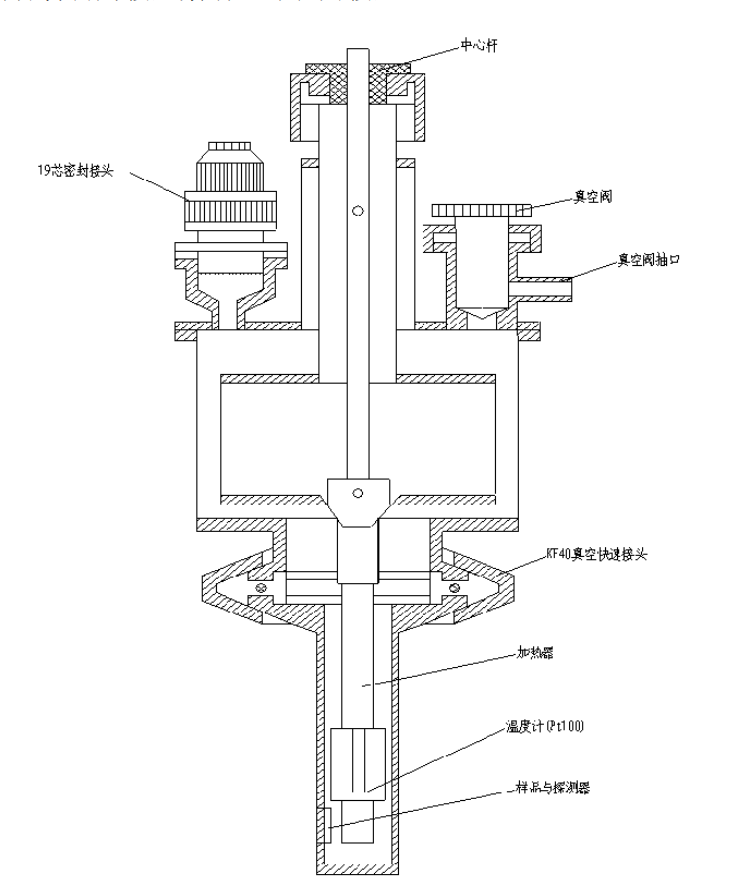
\includegraphics[width=0.6\linewidth]{pre1.png}
    \caption{漏热式液氮恒温器结构}
    \label{fig:cryostat}
\end{figure}

\subsubsection{强磁场技术}

实验中常用的人造强磁场包括脉冲磁场、超导磁场和电磁铁磁场。本实验采用电磁铁作为磁场源。

电磁铁由铁磁材料作为磁芯,外绕螺线管产生磁场。由于铁磁材料的高磁导率(约$10^3$量级),在较小电流下即可获得较强磁场。磁隙两侧通常设计成锥形以聚焦磁场,其极限磁感应强度取决于铁磁材料的饱和磁化强度,一般在数特斯拉范围。根据磁路定理,磁隙越宽,磁场强度越低。

出于安全考虑,实验室内电磁铁的磁感应强度通常限制在 0.6T 以内,实验区域内禁止存放无关物品或携带铁磁材料。由于铁磁性材料的磁滞效应,磁场与外加电流的对应关系并非严格线性,因此建议使用电源的磁场模式(FIELD),该模式具备自动消磁功能,并可借助特斯拉计测量磁场,精确控制磁感应强度。

液氮恒温器通常固定安装电磁铁,使样品位置相对磁隙稳定;对于循环制冷机恒温器,电磁铁可沿导轨水平移动,实验前需标定磁场与相对位置。

\subsubsection{电阻的测量}

\begin{itemize}
    \item \textbf{直流四引线测量电阻} 
    
    传统两引线测量方式不可避免地引入引线电阻和接触电阻,特别是在小电阻测量中误差较大。采用四引线法可以有效消除这些影响。由于电压表的输入阻抗较大(约$10^{10}\Omega$),流经测量引线的电流极小,因此接触电阻和引线电阻造成的电压降可忽略。
    
    \begin{figure}[h!]
        \centering
        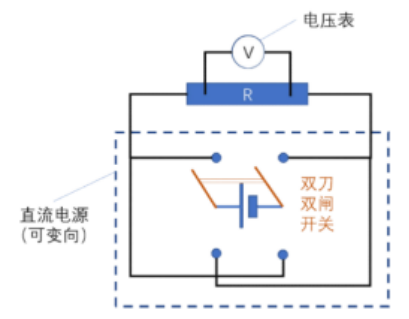
\includegraphics[width=0.6\linewidth]{pre2.png}
        \caption{直流四引线法测量电阻原理}
        \label{fig:4wire_dc}
    \end{figure}
    
    由于样品电极可能不对称,焦耳热、接触热阻以及温度梯度的不同可能引入温差电势和接触电势。直流四引线法通过反向电流测量来抵消这些误差,电阻计算公式如下:
    
    \begin{equation}
    R = \frac{V_+ - V_-}{2I}
    \end{equation}
    
    其中,$V_+$和$V_-$分别为正向与反向电流下的电压测量值。
    
    \item \textbf{交流四引线测量电阻} 
    
    交流测量方法可进一步消除温差电势和接触电势的影响。在交流测量中,通过测量电压有效值($V_{pp}/2\sqrt{2}$),可以获得交流电抗信息。
    
    \begin{figure}[h!]
        \centering
        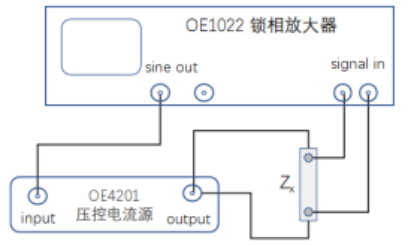
\includegraphics[width=0.6\linewidth]{pre3.png}
        \caption{交流四引线法测量电阻原理}
        \label{fig:4wire_ac}
    \end{figure}
    
    由于交流测量涉及容抗和感抗,测量频率的选择至关重要。锁相放大器可用于提高测量精度,并有效滤除噪声。然而,低频可能引入 $1/f$ 噪声,而过高频率可能导致引线寄生效应的影响。
    
    本实验电路采用交流压控电流源(最大输出 100mA),并使用锁相放大器(OE1022)进行电压采集,A、B 端采用差分输入方式。
    
\end{itemize}

\subsubsection{基于 LabVIEW 编程的实验管理}

实验中的低温与磁场系统由东方晨景提供,其温控和磁场控制模块已固定,支持 LabVIEW 驱动,可接受计算机指令,实现精准的温度与磁场控制。

本实验主要采用直流四引线法测量电阻,数据采集设备包括 NI PXIe4081、PXIe4083/4 和 IT6411S。

\subsubsection{超导电性简介}

超导是一种宏观量子现象,其本质是电子对(库珀对)的玻色-爱因斯坦凝聚。超导转变受温度、磁场和外加电流影响,可逆变换为正常态。

超导体具有两个基本特征:
\begin{itemize}
    \item \textbf{零电阻}:在超导态下,电阻降至零,电流可无损耗流动。
    \item \textbf{抗磁性(迈斯纳效应)}:超导体会排斥外部磁场,使磁感应强度在其内部趋于零。
\end{itemize}

外加磁场超过临界值时,超导性消失,电阻恢复正常。对于第二类超导体(Type-II),存在两个临界磁场,超导体在其间进入混合态,形成磁通涡旋。

高温超导指超导转变温度高于 BCS 理论极限(33K)的材料,其机制超出传统电声相互作用模型范畴。


\subsection{前思考题}
\begin{question}
    深低温系统为什么要抽真空?
\end{question}
深低温系统需要抽真空主要是为了减少热传导、热对流和热辐射,从而达到良好的隔热效果。在低温条件下,即使是极小的热量输入也可能导致温度上升,影响实验的精度和稳定性。

\begin{itemize}
    \item \textbf{减少气体传导漏热:}在大气环境下,气体分子通过碰撞传递热量。当系统被抽成真空后,气体分子数量显著减少,气体传导的热量大幅降低。
    \item \textbf{抑制热对流:}在有空气的情况下,热空气会上升,冷空气下沉,形成对流,导致热量传递。抽真空后,系统内部几乎没有空气,热对流基本消除。
\end{itemize}

\begin{question}
    真空泵产生一定的噪声,在达到真空要求后,是否可以关真空泵?关真空泵前,是否要先关真空阀门?
\end{question}
在达到真空要求后,可以关闭真空泵,但在关闭真空泵之前需要先关闭真空阀门。这样做的目的是:

\begin{itemize}
    \item \textbf{维持低温系统的真空状态:}如果先关闭真空泵而不关闭阀门,空气可能会通过泵逆流进入系统,破坏真空环境。
    \item \textbf{防止泵油或杂质进入系统:}某些类型的真空泵在停止工作后,可能会有微量油雾或杂质回流到系统内部,对实验环境造成污染。
\end{itemize}

\begin{question}
    为什么要安装屏蔽罩(防辐射屏)?屏蔽罩用哪一类材料最好?
\end{question}
屏蔽罩(防辐射屏)主要用于减少低温设备与环境之间的热辐射交换,降低热负载,以提高系统的制冷效率。

\begin{itemize}
    \item \textbf{屏蔽热辐射:}实验环境中,墙壁、设备和周围空气会向低温部分辐射热量,影响制冷效果。屏蔽罩可以阻挡和反射这些热辐射。
    \item \textbf{减少低温部件的热吸收:}采用高反射率的材料可以降低低温部件对环境辐射热的吸收,从而减小系统的稳态温度。
    \item \textbf{最佳材料选择:}本实验使用镀金紫铜作为屏蔽罩材料。紫铜具有良好的导热性能,可以快速均匀分布热量,而金的高反射率(尤其是在红外波段)能有效减少热辐射。
\end{itemize}
\begin{question}
    请估计直径为 12mm、长为 100mm,温度为 4K 的恒温器在无防辐射屏时的漏热约为多
少?在采用一层防辐射屏后,其与环境之间的辐射漏热减少了多少?如果将防辐射屏的温
度降到液氮温度(77K),则该防辐射屏的辐射漏热又为多少?
\end{question}

假设恒温器为圆柱体,直径为 12mm,长度为 100mm,温度为 4K,环境温度为 300K。我们计算其辐射漏热。

首先,计算圆柱体的表面积。圆柱的半径为:
\[
r = \frac{12\,\text{mm}}{2} = 6\,\text{mm} = 0.006\,\text{m}
\]
圆柱的长度为:
\[
L = 100\,\text{mm} = 0.1\,\text{m}
\]

圆柱的表面积由侧面和两个底面组成:
\[
A_{\text{side}} = 2\pi r L = 2\pi(0.006\,\text{m})(0.1\,\text{m}) = 0.00377\,\text{m}^2
\]
\[
A_{\text{top/bottom}} = \pi r^2 = \pi(0.006\,\text{m})^2 = 1.13 \times 10^{-4}\,\text{m}^2
\]
总表面积为:
\[
A = A_{\text{side}} + 2 \times A_{\text{top/bottom}} = 0.00377\,\text{m}^2 + 2 \times 1.13 \times 10^{-4}\,\text{m}^2 = 0.004\,\text{m}^2
\]

根据斯图尔特–玻尔兹曼公式计算辐射热流:
\[
Q = \sigma A \epsilon (T^4 - T_0^4)
\]
其中,\(\sigma = 5.67 \times 10^{-8}\,\text{W/m}^2\text{K}^4\),
\(T = 4\,\text{K}\),\(T_0 = 300\,\text{K}\),\(\epsilon = 1\)。
代入计算:
\[
Q \approx 1.84\,\text{W}
\]


假设防辐射屏的发射率非常低(接近 0),能够显著减少辐射热流。因此,辐射漏热将大大减少。

若防辐射屏温度降至 77K,使用同样的公式计算:
\[
Q_{\text{screen}} \approx 1.83 \times 10^{-3}\,\text{W}
\]

\subsection*{总结}

\begin{itemize}
    \item 无防辐射屏时的辐射漏热约为 1.84 W。
    \item 加入防辐射屏后,当屏幕温度降至 77K 时,辐射漏热降至约 0.00183 W。
\end{itemize}

\begin{question}
    铂电阻温度计位置不在样品旁边,有什么因素会影响样品温度偏离温度计的温度?偏离有多大?能否测量或通过建模进行定量分析?
\end{question}
温度计与样品之间存在温度偏差的主要影响因素包括:
\begin{enumerate}
    \item \textbf{热传导阻抗}:样品与温度计之间的热连接方式及其热阻会影响温度的传递。连接材料的导热系数、接触热阻以及安装方式都可能导致温度差异。
    \item \textbf{热容效应}:如果样品和温度计的热容相差较大,在温度变化过程中可能会出现温度滞后,导致两者的瞬时温度不同。
    \item \textbf{寄生热流}:周围环境(如支架、样品台、引线)可能通过热传导或辐射方式影响样品,使其温度与温度计不同。
    \item \textbf{环境温度波动}:实验环境的温度变化可能导致温度计和样品的热交换不同步,造成测量误差。
\end{enumerate}

温度偏差的大小可以通过稳态热传导方程估计:
\begin{equation}
    \Delta T = \frac{P_{\text{loss}}}{K_{\text{eff}}}
\end{equation}
其中 $P_{\text{loss}}$ 为寄生热流,$K_{\text{eff}}$ 为温度计与样品之间的有效热导率。对于低温实验,可以使用有限元分析(FEM)或热传导模型进行建模分析,并通过实验测量(如热响应时间对比、热传导校准)进行验证和修正。

\begin{question}
    高磁场下电磁铁长时间工作会导致线圈温度升高,如何在满足实验需求的同时,使线圈电流最小、且实验时间最短?然后如何保护自己避免烫伤、又不影响线圈散热?
\end{question}

\textbf{优化实验参数以降低线圈温升}:
\begin{enumerate}
    \item 计算实验所需的最低磁场,并选择对应的最小电流,避免过高电流造成不必要的功耗;
    \item 采用合理的工作-休息周期,避免线圈长时间连续工作导致过热;
    \item 预先准备好实验流程和设备,减少实验过程中电磁铁的工作时间;
    \item 采用低电阻、高导热率的线圈材料(如铜线),降低焦耳热产生;
    \item 若条件允许,可使用脉冲磁场代替持续磁场,以减少功耗和发热。
\end{enumerate}

\textbf{安全防护与散热措施}:
\begin{enumerate}
    \item 在电磁铁周围安装强制风冷系统或水冷系统,提高散热效率;
    \item 避免直接接触电磁铁线圈,可使用耐高温手套或隔热工具;
    \item 在实验区域设置高温警告标识,提醒实验人员注意安全;
    \item 确保线圈周围的空气流通,避免阻挡散热通道,如避免密封电磁铁外壳;
    \item 在实验过程中监测线圈温度,若温度超限,则暂停实验并让线圈冷却。
\end{enumerate}


\begin{question}
    本实验中样品位置的磁场与霍尔探头测量的磁场有多大的偏差?如何校正?校正时电磁铁电源能选用“磁场模式”吗?为什么?
\end{question}

\textbf{磁场测量偏差的来源}:
\begin{enumerate}
    \item 霍尔探头的测量点与样品位置存在空间偏移,导致测量磁场与样品实际磁场不同;
    \item 由于磁场不完全均匀,磁隙内不同位置的磁场强度可能存在梯度;
    \item 霍尔探头的零点漂移或非线性误差可能导致测量值偏差。
\end{enumerate}

\textbf{磁场校正方案}:
\begin{enumerate}
    \item 在不同位置测量磁场分布,绘制磁场梯度图,确定样品位置的实际磁场;
    \item 采用磁通计或 NMR 磁强计对霍尔探头测量进行标定,提高测量准确性;
    \item 通过有限元模拟计算磁场分布,并与实验测量进行对比,修正偏差。
\end{enumerate}

\textbf{是否可以使用“磁场模式”进行校正?}:

   可以,因为磁场模式采用反馈控制,能通过测量的磁场值调节电流,使磁场更加稳定和可控;若霍尔探头位置与样品不同,磁场模式可能基于探头位置调整电流,导致样品位置磁场仍有偏差,因此仍需额外校正。




\begin{question}
    如果采用“磁场模式”加磁场,会有剩磁问题吗?
\end{question}

\textbf{磁场模式的剩磁特性}:
\begin{itemize}
    \item 磁场模式带有自动消磁功能,能在设定磁场归零时,逐步降低电流并消除剩磁;
    \item 可使用高斯计检查剩磁,并在必要时手动执行额外的消磁步骤。
\end{itemize}





\begin{question}
    外加磁场与电流方向的夹角不同,洛伦兹力不同,从而超导体的磁流阻大小不同。针对研究磁场(矢量)对超导转变的影响,写出你的实验方案。
\end{question}

研究超导体在不同方向外加磁场下的超导转变特性,探究磁流阻的各向异性及磁场对超导态稳定性的影响。
\textbf{实验装置与测量方法}:
\begin{itemize}
    \item 采用低温恒温器(液氮系统)提供稳定低温环境;
    \item 采用三轴磁铁或旋转样品台,以控制磁场方向;
    \item 采用四引线法测量样品的电阻,并结合锁相放大器提高信噪比;
    \item 记录不同磁场方向(相对于电流)的临界磁场、超导转变温度及磁流阻;
    \item 通过特斯拉计测量实际磁场分布,并校正样品的取向误差。
\end{itemize}

\textbf{数据分析}:
\begin{itemize}
    \item 研究磁场方向对超导转变温度的影响;
    \item 计算各向异性参数,分析磁通运动与洛伦兹力的关系;
\end{itemize}



\begin{question}
    用直流法和交流法测量电阻有何差异?对于交流法测量电阻,是否可以有效地扣除测量系统中感抗和容抗的贡献?如何扣除?
\end{question}

\textbf{直流法 vs. 交流法}:
\begin{itemize}
    \item 直流法通过恒流源施加电流,测量电压并计算电阻,适用于大多数金属和半导体;
    \item 交流法采用锁相放大器,可有效抑制低频噪声,提高测量微小电阻的精度;
    \item 交流法可通过相敏检测,分离出样品的阻性、感抗和容抗成分。
\end{itemize}

\textbf{扣除感抗和容抗的方法}:
选择合适的测量频率,使感抗和容抗的影响最小;通过锁相放大器的相敏检测功能,仅提取与电流同相的信号分量(即纯电阻部分);进行背景测量,记录连接导线及仪器内部的寄生电抗,并进行补偿。



\begin{question}
    与标准四引线法(四电极)相比,两电极四引线有何不同,并说明在超导态能否测出零电阻。
\end{question}

\textbf{两电极四引线 vs. 标准四引线}:
\begin{itemize}
    \item 标准四引线法(四电极)采用独立的电流和电压测量引线,可有效消除接触电阻影响;
    \item 两电极四引线法在样品两端接有公共电极,测量信号仍然会受到接触电阻的影响。
\end{itemize}

\textbf{在超导态的测量问题}:
\begin{itemize}
    \item 在超导态,理想情况下超导体应呈零电阻;
    \item 若使用四电极法,则测量的电压降为零,可以确定超导转变;若使用两电极四引线法,由于接触电阻的存在,测得的电压可能非零,导致测量误差;
    \item 可以通过 I-V 特性测试超导跃迁点,以更准确判断超导态的形成。
\end{itemize}




\subsection{第二周实验的实验方案}
\subsubsection{实验目的}
本实验旨在探究外加磁场如何影响超导转变时电阻随温度的变化。通过精确测量样品在不同磁场条件下的超导转变温度,并分析其变化趋势,以深入理解磁场对超导体电子态的影响。

\subsubsection{实验设备}
\begin{itemize}
    \item 低温系统(包含液氮恒温器)
    \item 交流四引线测量系统(电流源、纳伏表)
    \item LabVIEW 控制系统
    \item 电磁铁及电源
    \item 真空系统(机械泵、真空阀等)
    \item 温度控制系统(控温仪、温度计)
\end{itemize}

\subsubsection{实验准备}
\begin{enumerate}
    \item 确认真空球阀处于关闭状态,检查样品罩、机械泵等处的卡箍是否闭紧。
    \item 关闭真空阀后,打开真空泵并运行至少 2 分钟,确保无明显的“呼噜”声后,缓慢旋转打开真空阀至完全打开,使系统抽真空。
    \item 真空泵运行 20 分钟后,逆时针旋转丝杆至“液氮针阀”完全打开,并使用漏斗向制冷仪内注入液氮,直到有少量液氮漏出。
    \item 注入完毕后,用纱布将排气孔裹住,防止空气进入冷凝水凝固堵塞针阀。
    \item 当温度降至200K附近时,关闭真空阀,并关闭真空泵。
    \item 使用LabVIEW程序控制温度,选择合适的挡位和调整丝杆高度,从而达到所需的升降温速率。
\end{enumerate}

\subsubsection{实验过程}
\begin{enumerate}
    \item 使用交流四引线法测量电阻,通过LabVIEW程序实现实时的电阻测量,对于温度可以考虑进行已标定电阻的温度换算。
    \item 设置外加磁场梯度,重复步骤1,测量得到不同外磁场条件下的超导转变温度。
    \item 记录超导转变温度随外磁场强度的变化,绘制曲线并分析数据。
\end{enumerate}
